\chapter{Úvod}
\label{sec:Introduction}

\begin{figure}[H]
\centering
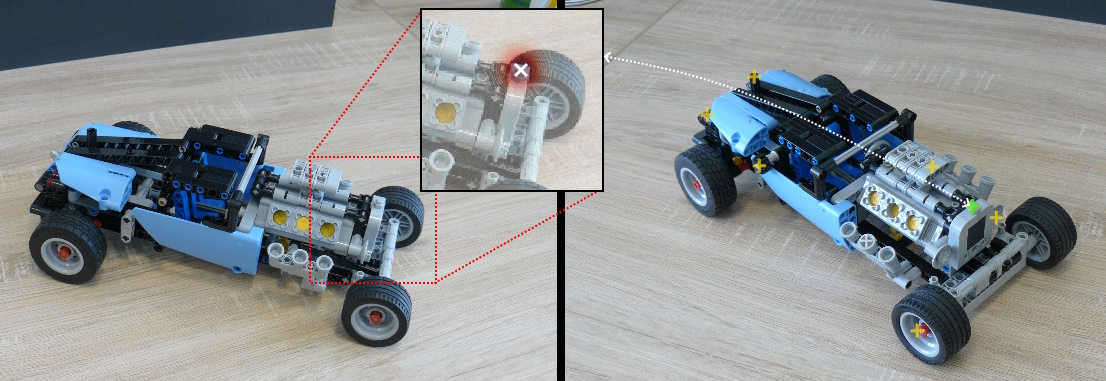
\includegraphics[width=1.0\textwidth,keepaspectratio]{Figures/bp_uvodni_obrazek.jpg}
\caption[Lokalizace klíčového bodu pro řešení PnP problému]{Lokalizace jednoho z klíčových bodů pro řešení PnP problému mezi reálným snímkem (vlevo) a syntetickým vykreslením (vpravo) se známými pozicemi klíčových bodů.}
\label{fig:bp_uvodni_obrazek}
\end{figure}


Lokalizace klíčových bodů zůstává nadále jedním z aktivně řešených problémů analýzy obrazu dnešní doby.
Klíčové body chápeme jako konkrétní body nacházející se na objektu zájmu, které chceme lokalizovat a následně sadu nalezených klíčových bodů použít pro další zpracování tykající se daného objektu zájmu, či jeho částí.

Využití lokalizace bodů nacházíme kupříkladu při odhadu postoje osob \cite{humanpose} nebo v biomedicínské technice \cite{unet}.
Při jejich následné lokalizaci musíme počítat s několika kvalitativně ovliňujícími členy v obrazu jako např. natočení kamery, vzdálenost, osvětlení, charakteristiky a kvalitu obrazu (zaostření) a ostatní vlivy prostředí okolo klíčového bodu. Kvůli tomuto musí techniky pro lokalizaci klíčových bodů být invariantní (tj. odolné vůči změnám ve vzhledu objektů), aby mohly spolehlivě fungovat i během změn vnějších podmínek mezi různými obrazy.

Cílem této bakalářské práce je využít techniky lokalizace klíčových bodů pomocí hlubokých sítí U-Net (a jejími následovníky či variacemi) pro zpřesnění 6 stupňů volnosti (DoF) transformace cílového objektu ve 3D prostoru pomocí PnP metod. PnP metody představují výpočetní techniky určené k řešení PnP problémů, které se zaměřují na přesný odhad polohy a orientace 3D objektů na základě korespondence lokalizovaných klíčových bodů na 2D snímku a známých pozicích klíčových bodů na 3D objektu.

Úloha lokalizace pro část vstupního snímku obsahující klíčový bod je ilustrována pomocí obrázku \ref{fig:bp_uvodni_obrazek}. Pro objekt byl detekován hrubý odhad pozice klíčového bodu. Klíčový bod je pomocí hluboké konvoluční neuronové sítě korektně lokalizován na lokaci s globálním maximem výsledku skalárního pole. Klíčový bod také byl korektně klasifikován s třídou známého klíčového bodu. Za předpokladu korektní lokalizace dostatečného počtu klíčových bodů můžeme orientaci objektu z levé části snímku odhadnout a vyjádřit pomocí 6 stupňů volnosti (DoF).

Výsledná metoda by následně měla být použita pro příjem proud RGB dat z kamery a správně odhadovat pózu objektu v reálném čase. Naše metody řešení budou trénovány na syntetickém datasetu klíčových bodů objektu zájmu a následně porovnány mezi sebou.
\endinput